% Pipeline figure for Section~\ref{sec:method}: flow of the 731 tasks.
% Band and bar heights are proportional to task counts (0.046 mm per task).
% Preamble: \usepackage{tikz,graphicx} (xcolor is loaded by tikz)
\definecolor{sbpFlag}{HTML}{4C72B0}
\definecolor{sbpRep}{HTML}{55A868}
\definecolor{sbpDisc}{HTML}{C44E52}
\definecolor{sbpKeep}{HTML}{7F7F7F}
\definecolor{sbpNone}{HTML}{B0B0B0}
\begin{figure*}[t]
\centering
\resizebox{\textwidth}{!}{%
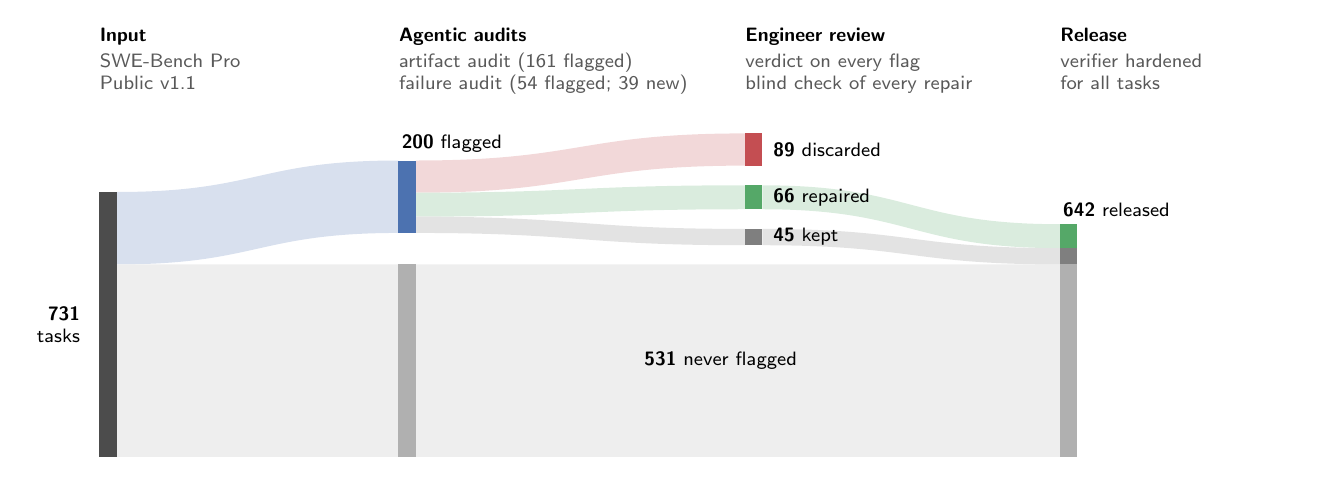
\begin{tikzpicture}[x=1mm, y=1mm, font=\sffamily\scriptsize,
  execute at begin node={\hyphenpenalty=10000\exhyphenpenalty=10000}]
% flagged by an audit
\fill[sbpFlag!22] (2.2,4.09) .. controls (20.1,4.09) and (20.1,8.09) .. (38,8.09)
  -- (38,-1.11) .. controls (20.1,-1.11) and (20.1,-5.11) .. (2.2,-5.11) -- cycle;
% never flagged
\fill[sbpNone!22] (2.2,-5.11) .. controls (20.1,-5.11) and (20.1,-5.11) .. (38,-5.11)
  -- (38,-29.54) .. controls (20.1,-29.54) and (20.1,-29.54) .. (2.2,-29.54) -- cycle;
% discarded
\fill[sbpDisc!22] (40.2,8.09) .. controls (61.1,8.09) and (61.1,11.53) .. (82,11.53)
  -- (82,7.44) .. controls (61.1,7.44) and (61.1,4) .. (40.2,4) -- cycle;
% repaired
\fill[sbpRep!22] (40.2,4) .. controls (61.1,4) and (61.1,4.94) .. (82,4.94)
  -- (82,1.9) .. controls (61.1,1.9) and (61.1,0.96) .. (40.2,0.96) -- cycle;
% kept unchanged
\fill[sbpKeep!22] (40.2,0.96) .. controls (61.1,0.96) and (61.1,-0.6) .. (82,-0.6)
  -- (82,-2.67) .. controls (61.1,-2.67) and (61.1,-1.11) .. (40.2,-1.11) -- cycle;
% never flagged, passes review
\fill[sbpNone!22] (40.2,-5.11) .. controls (81.1,-5.11) and (81.1,-5.11) .. (122,-5.11)
  -- (122,-29.54) .. controls (81.1,-29.54) and (81.1,-29.54) .. (40.2,-29.54) -- cycle;
% repaired -> release
\fill[sbpRep!22] (84.2,4.94) .. controls (103.1,4.94) and (103.1,0) .. (122,0)
  -- (122,-3.04) .. controls (103.1,-3.04) and (103.1,1.9) .. (84.2,1.9) -- cycle;
% kept -> release
\fill[sbpKeep!22] (84.2,-0.6) .. controls (103.1,-0.6) and (103.1,-3.04) .. (122,-3.04)
  -- (122,-5.11) .. controls (103.1,-5.11) and (103.1,-2.67) .. (84.2,-2.67) -- cycle;
% nodes
\fill[black!70] (0,-29.54) rectangle (2.2,4.09);
\fill[sbpFlag] (38,-1.11) rectangle (40.2,8.09);
\fill[sbpNone] (38,-29.54) rectangle (40.2,-5.11);
\fill[sbpDisc] (82,7.44) rectangle (84.2,11.53);
\fill[sbpRep] (82,1.9) rectangle (84.2,4.94);
\fill[sbpKeep] (82,-2.67) rectangle (84.2,-0.6);
\fill[sbpRep] (122,-3.04) rectangle (124.2,0);
\fill[sbpKeep] (122,-5.11) rectangle (124.2,-3.04);
\fill[sbpNone] (122,-29.54) rectangle (124.2,-5.11);
% labels
\node[anchor=east, align=right] at (-1.2,-12.72) {\textbf{731}\\tasks};
\node[anchor=south west, inner sep=1pt] at (38,8.69) {\textbf{200} flagged};
\node[anchor=west] at (68,-17.32) {\textbf{531} never flagged};
\node[anchor=west, inner sep=1pt] at (85.2,9.48) {\textbf{89} discarded};
\node[anchor=west, inner sep=1pt] at (85.2,3.42) {\textbf{66} repaired};
\node[anchor=west, inner sep=1pt] at (85.2,-1.64) {\textbf{45} kept};
\node[anchor=south west, inner sep=1pt] at (122,0.6) {\textbf{642} released};
% stage headers
\node[anchor=north west, inner sep=0pt, text width=34mm, align=left] at (0,25.03)
  {{\bfseries Input}\\[1.5pt]\textcolor{black!65}{SWE-Bench Pro\\Public v1.1}};
\node[anchor=north west, inner sep=0pt, text width=43mm, align=left] at (38,25.03)
  {{\bfseries Agentic audits}\\[1.5pt]\textcolor{black!65}{artifact audit (161 flagged)\\failure audit (54 flagged; 39 new)}};
\node[anchor=north west, inner sep=0pt, text width=38mm, align=left] at (82,25.03)
  {{\bfseries Engineer review}\\[1.5pt]\textcolor{black!65}{verdict on every flag\\blind check of every repair}};
\node[anchor=north west, inner sep=0pt, text width=30mm, align=left] at (122,25.03)
  {{\bfseries Release}\\[1.5pt]\textcolor{black!65}{verifier hardened\\for all tasks}};
\end{tikzpicture}}%
\caption{Flow of the 731 tasks; bar and band heights are proportional to
task counts. The artifact audit (an LLM agent and a human auditor compare the
instruction with the tests and reference patch) and the failure audit (an LLM
judge attributes failed runs of four agent setups) flag 200 tasks. Engineers
adjudicate every flag, and a repair ships only after a blind re-implementation
of the edited instruction passes the hidden tests.}
\label{fig:pipeline}
\end{figure*}
